\section{Subration}

I recently pulled out a couple of old books and notes from a box packed up years ago. One is \emph{Advaita Vedanta: A Philosophical Reconstruction} by the philosopher \textbf{Eliot Deutsch}. In reformulating Vedantic metaphysics in Western categories, he brings up some useful points. One is the idea of “subration” which he uses to translate the Sanskrit term \emph{badha}. He defines it thus:

\begin{quotex}
\emph{Subration} is the mental process whereby one disvalues some previously appraised object or content of consciousness because of its being contradicted by a new experience. A judgment about something is contradicted by a new experience when it is impossible to affirm both the previous judgment and what is learned or acquired in the new experience. … An object or content of consciousness is \emph{subrated} or \emph{subratable} when it is or can be disvaluated, denied, or contradicted by another experience. 

\end{quotex}
He applies that definition to different levels of being as described in the Vedanta.

\begin{itemize}
\item \textbf{Appearance} is that which can be subrated by another experience. 
\item \textbf{Reality} is that which cannot be subrated by any other experience. 
\item \textbf{Nonbeing} is that which neither can nor cannot be subrated by other experience. 
\end{itemize}
Subration involves:

\begin{enumerate}
\item A judgment about some object of content of consciousness (thing, person, place, condition, idea) 
\item The recognition, in the light of another kind of judgment that is incompatible with the initial judgment, that the initial judgment is faulty 
\item The acceptance of the new judgment as valid 
\end{enumerate}
How is this related to levels of being? Professor Deutsch points out that the more something is subratable, the less being it has. Clearly, then, the level of being corresponds to the level of knowledge. When we are asked judge not by appearances, but by a just judgment, we are asked to move from appearance to reality. Although Professor Deutsch provides detailed and subtle examples of the various levels and sublevels of being, we are cutting to the basics for now because we are more interested in relating them to esoteric experiences in particular.

\paragraph{Appearance}
There are three types of existents which account for appearances.

\begin{itemize}
\item \textbf{Illusory existent}. This comprises those contents of experience that can be subrated by all other types of experience. E.g., hallucinations, fantasies, daydreams, erroneous sense perceptions, false, inconsistent, incoherent, contradictory theories or concepts. They have no relationship to what is real. 
\item \textbf{Ordinary existent}. This can be subrated by other existents or Reality. 
\item \textbf{Real existent}. This can be subrated only by Reality. 
\end{itemize}
The first focus must be the overcoming of illusion, since they absorb psychic energy while bringing us no closer to reality. We are buffeted by illusory inputs which challenge our opinions. But rather than subrating them, we protect ourselves with more complex theories or else hang on more tightly to established opinions. That is why esoteric work begins with the tedious process of breaking down our false self images through intense practice of self observation.

Ordinary existents are not as much false as they are incomplete. For example, we may engage in a relationship of convenience, thinking it is the real thing, yet it falls well short of a true spiritual friendship.

Or we may take things to be independent, failing to discern how they are part of a larger whole.

A real existent is the highest level of the experience of appearances since it cannot be contradicted by other experiences. We know a real existent by discursive thought, i.e., dualistically. This knowledge is subrated by non-dual knowledge.

\paragraph{Reality}
While illusory existents are mere mental artifacts and have no reality at all, the other categories of appearances do participate in reality. Specifically, they are possibilities of manifestation as manifested. Because of privation, they may not be properly recognized. But to know them is to know the idea of them. Since reality cannot be contradicted, it is non-dual. That is, “knowing is being”. When I know the idea of a thing, I \emph{am} that thing, at least in essence, since its idea is in my mind.

There are more and more comprehensive notions of the real, each higher level incorporating the lower into a larger whole, until Being itself is reached.

\paragraph{Nonbeing}
Prof Deutsch calls this “unreality”, although I prefer \textbf{Rene Guenon}'s usage for reasons that follow. Prof Deutsch includes in this category self-contradictory concepts, such as a “square circle”, which cannot be manifested. However, the category of nonbeing includes more than that. For example, Guenon mentions the Void and the Silence as other possibilities of non-manifestation. Another example is Chaos. These are pure privation with no actuality at all. Hence, we could include evil, death, and disease in this category. Being itself is part of nonbeing.

\paragraph{Influences}
At every moment, we are being exposed to two types of influences:

\begin{itemize}
\item Illusory influences, or “A” influences for short. 
\item Real influences, or “B” influences. 
\end{itemize}

\begin{wrapfigure}{rt}{0.35\textwidth}
 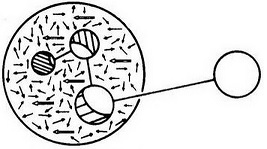
\includegraphics[scale=.6]{a20141010Subration-img001.jpg}
\end{wrapfigure} 

Their action is illustrated in the diagram on the right, taken from \emph{Gnosis} by \textbf{Boris Mouravieff}. The A influences come from every direction and their net, or vector sum, is zero. Although we may be temporarily in a region of similar A influences, overall, they subrate each other and lead nowhere.

The B influences (represented by the thicker arrows), on the other hand, are consistent and flow in the same direction. These are our encounters with the Real. Hence, the next step in esoteric training is to be vigilant in watching the thoughts that we entertain in our mind. We learn to discard the A influences, while allowing in the B influences.

\paragraph{Science of Being}

\begin{wrapfigure}{rt}{0.35\textwidth}
 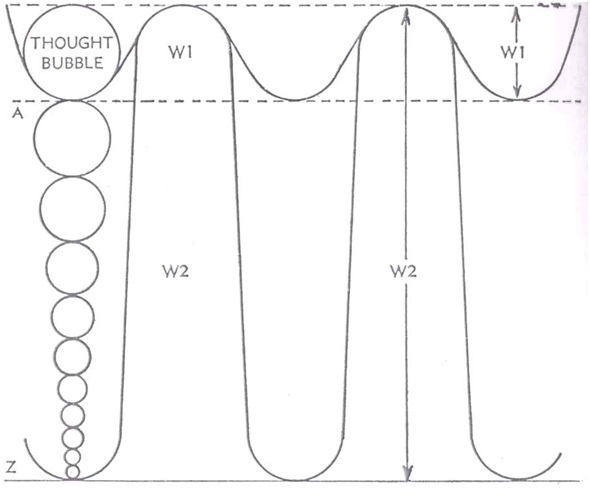
\includegraphics[scale=.35]{a20141010Subration-img002.jpg}
\end{wrapfigure} 

In the same box, I found a yellowing copy of \emph{The Science of Being and the Art of Living}, by \textbf{Maharishi Mahesh Yogi}. Published around the same time as the Deutsch book, it was my initial exposure to Vedantic teachings. Although he was non-traditional in important respects (which we can't get into just now), he was nevertheless well versed in Vedantic doctrines. Since he did propose a path of self-development while being active in the world, he is of a certain interest. In particular, I want to point to a diagram that may help in the process of moving from ordinary to real existents, and then to reality itself.

The goal of vigilance is to improve the quality of thoughts. The Maharishi writes:

\begin{quotex}
The art of thinking should mean that the manner of thinking is such that the least amount of mental energy is consumed … the thought should not only be powerful but it should be right as well. The art of thinking also means that no useless or wrong thought should occupy the mind. 

\end{quotex}
In esoteric training, we learn to observe thoughts. Ordinarily, we become aware of a thought only when it has become fully formed. At that point, further thoughts arise and start linking with each other. At that point we tend to lose full consciousness and become “lost in thought”.

However, by remaining conscious, we may be able to discern the thought in its formation process. This is like bubbles arising; awareness will keep the thought from fully arising. By going into deeper levels of being, we may be able to move beyond the thought into nondual awareness.


\hfill

\flrightit{Posted on 2014-10-10 by Cologero }

\begin{center}* * *\end{center}

\begin{footnotesize}\begin{sffamily}

\texttt{David on 2014-10-21 at 00:46 said: }

Greetings Colgero. A question regarding nonbeing. Could you develop more around it ? My understanding of it was mostly based on Eckhart works, and I was under the impression that for him Non-Being was at the center of creation, from which Being sprung forth and was unknowable. 

The diagram with the arrows is quite simple, yet very effective. I will have to meditate on that. 

Thank you.


\hfill

\texttt{Cologero on 2014-10-22 at 00:37 said: }

Synchronistically, David, a post on that topic has been planned in regards to the Ray of Creation or Great Chain of Being. Your description from Eckhart sounds compatible with what Guenon writes in the Multiple States of Being.


\end{sffamily}\end{footnotesize}
